\section*{Programming Model}

\begin{lstlisting}[language=C++, caption={C++ code using listings}]
int main()
{
    // print hello to the console
    std::cout << "Hello, world!" << std::endl;
    return 0;
}
\end{lstlisting}

\subsection*{Runtime Model}

\subsection*{Control Model}

Figure \ref{fig:cycle} shows...

\begin{figure}
\begin{center}
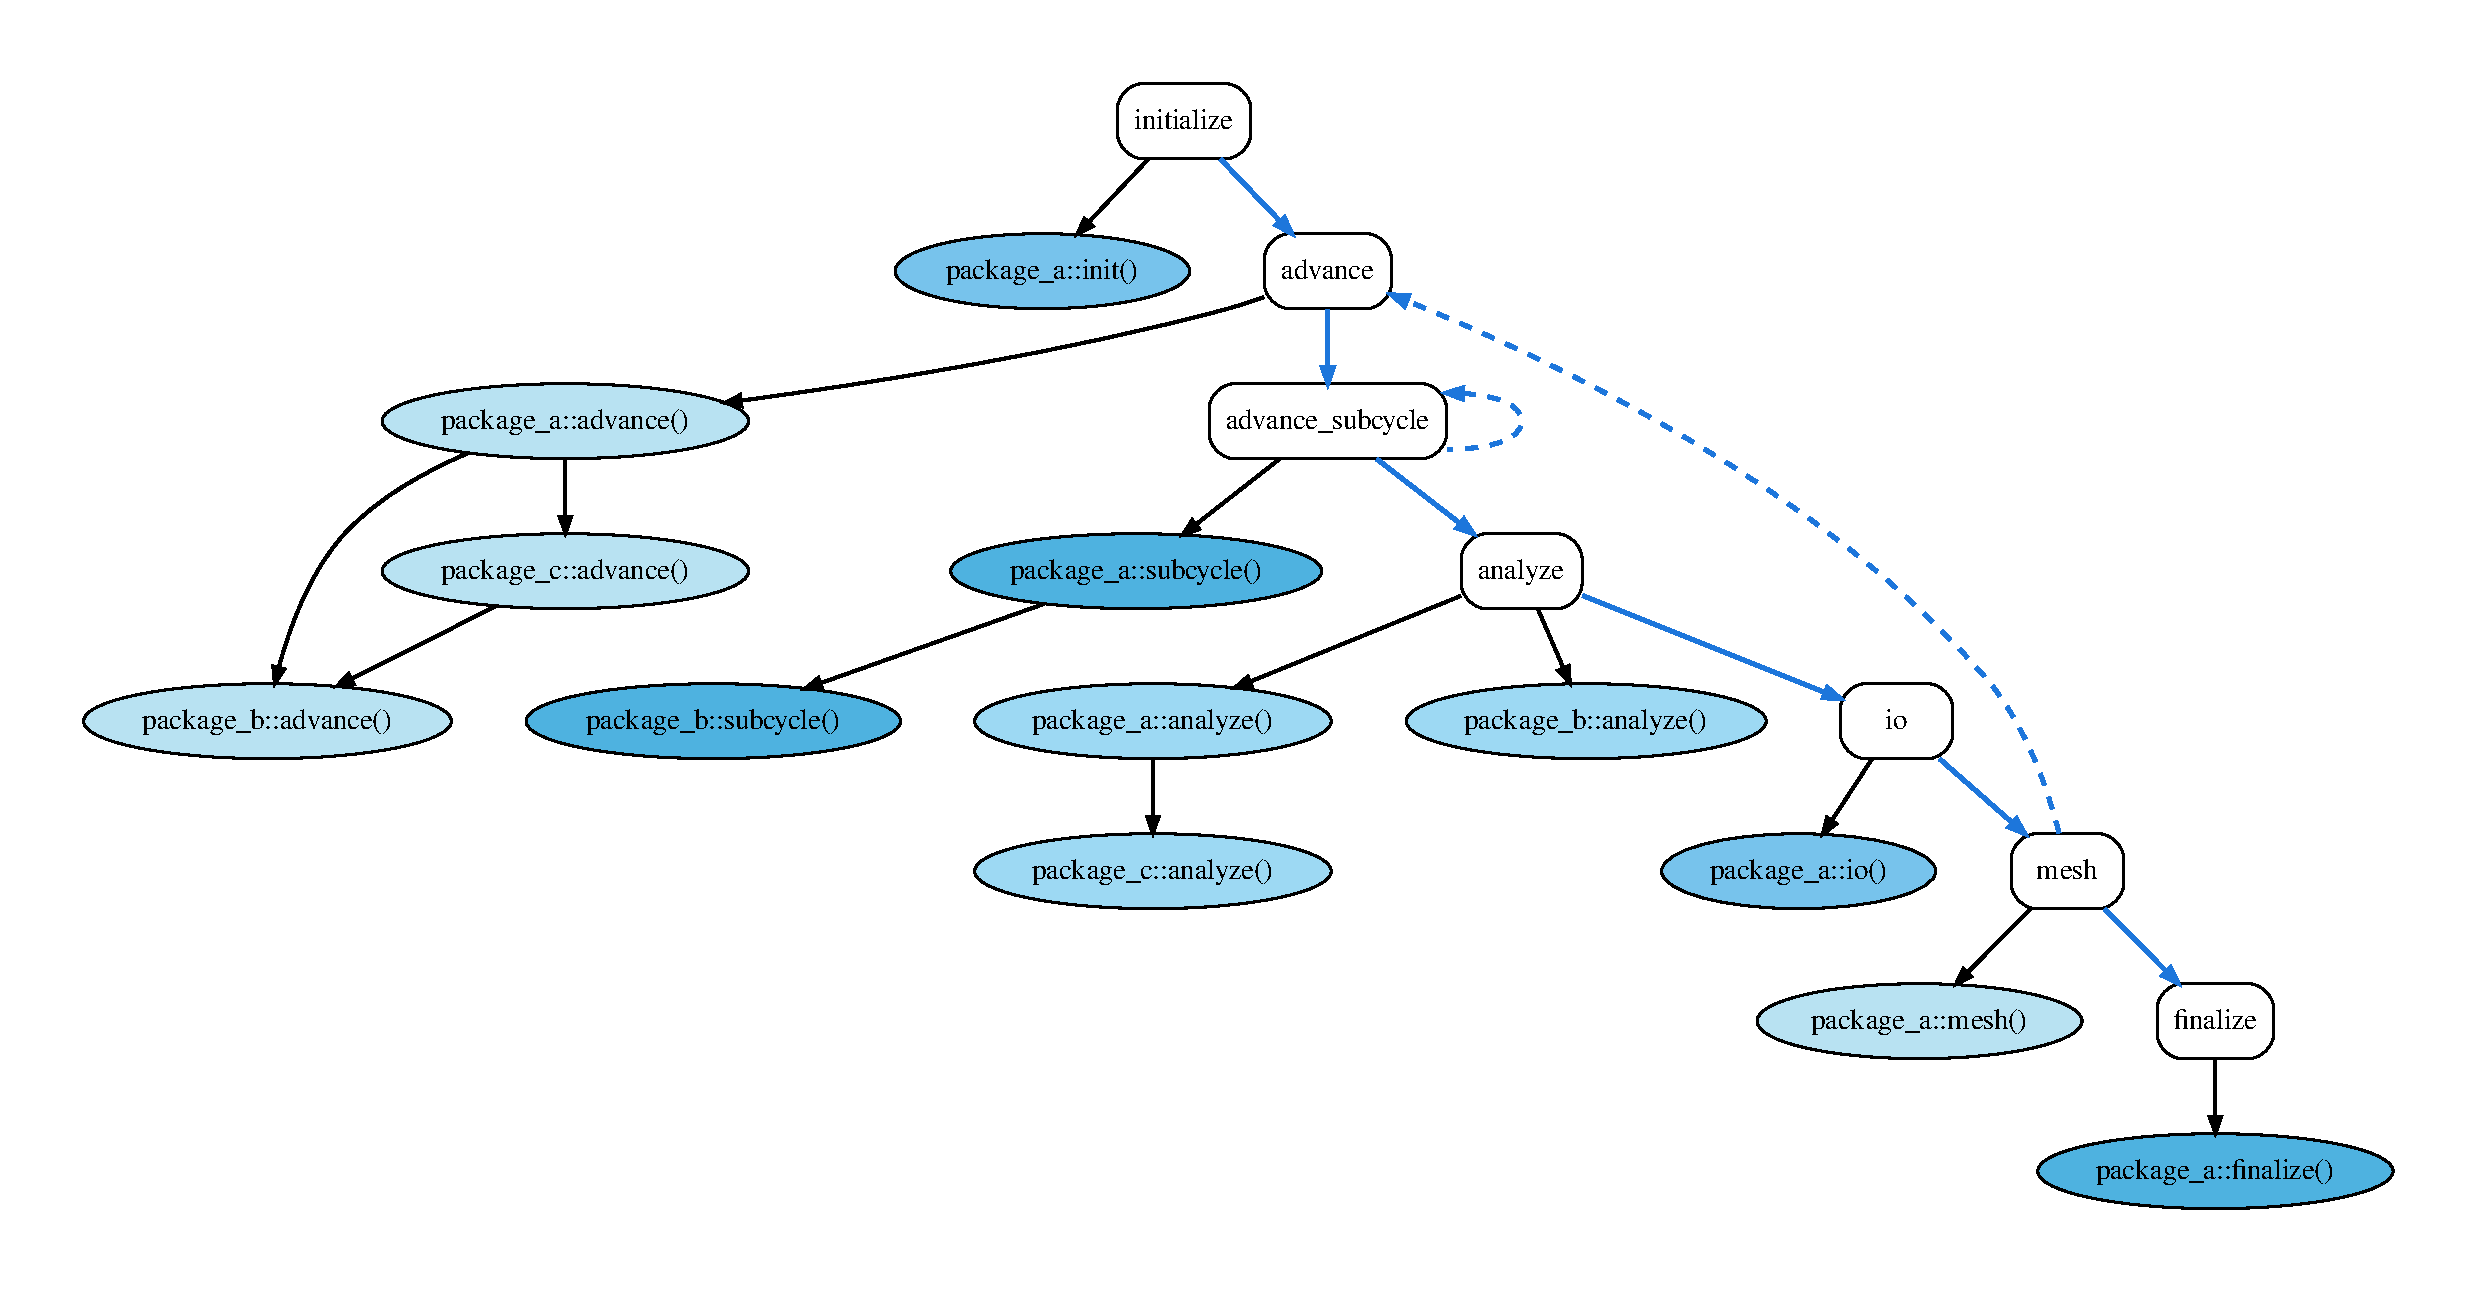
\includegraphics[width=1.0\textwidth]{images/cycle.pdf}
\end{center}
\caption{This is a pdf figure.}
\label{fig:cycle}
\end{figure}

\subsection*{Data Model}

\subsection*{Execution Model}

% vim: set tabstop=2 shiftwidth=2 expandtab fo=cqt tw=72 :
